\let\negmedspace\undefined
\let\negthickspace\undefined
\documentclass[journal]{IEEEtran}
\usepackage[a5paper, margin=10mm, onecolumn]{geometry}
%\usepackage{lmodern} % Ensure lmodern is loaded for pdflatex
\usepackage{tfrupee} % Include tfrupee package

\setlength{\headheight}{1cm} % Set the height of the header box
\setlength{\headsep}{0mm}     % Set the distance between the header box and the top of the text
\usepackage{gvv-book}
\usepackage{gvv}
\usepackage{cite}
\usepackage{amsmath,amssymb,amsfonts,amsthm}
\usepackage{algorithmic}
\usepackage{graphicx}
\usepackage{textcomp}
\usepackage{xcolor}
\usepackage{txfonts}
\usepackage{listings}
\usepackage{enumitem}
\usepackage{mathtools}
\usepackage{gensymb}
\usepackage{comment}
\usepackage[breaklinks=true]{hyperref}
\usepackage{tkz-euclide} 
\usepackage{listings}
% \usepackage{gvv}                                        
\def\inputGnumericTable{}                                 
\usepackage[latin1]{inputenc}                                
\usepackage{color}                                            
\usepackage{array}                                            
\usepackage{longtable}                                       
\usepackage{calc}                                             
\usepackage{multirow}                                         
\usepackage{hhline}                                           
\usepackage{ifthen}                                           
\usepackage{lscape}
\begin{document}

\bibliographystyle{IEEEtran}
\vspace{3cm}

\title{9.3.12B}
\author{EE24BTECH11027 - satwikagv}
% \maketitle
% \newpage
% \bigskip
{\let\newpage\relax\maketitle}

\renewcommand{\thefigure}{\theenumi}
\renewcommand{\thetable}{\theenumi}
\setlength{\intextsep}{10pt} % Space between text and floats


\numberwithin{equation}{enumi}
\numberwithin{figure}{enumi}
\renewcommand{\thetable}{\theenumi}
\textbf{Question}:\\
Plot the solution of the differential equation: 
\begin{align}
    y^{\prime\prime} +xy^\prime + xy = x. 
\end{align}
\textbf{Solution}:\\
To plot the curve of the given differential equation $\brak{0.1}$ we can do it using the method of finite differences which is a numerical technique for solving complex differential equations by approximating derivatives with differences.\\
The approximated forward derivative of $y\brak{x}$ is given as:\\
\begin{align}
    y^\prime_n\approx\frac{y_{n+1}-y_n}{h}
\end{align}
On rearranging we get,
\begin{align}
    y_{n+1}=y_n+y^\prime_n\brak{h}
\end{align}
And also 
\begin{align}
    x_{n+1}=x_n+h
\end{align}
The approximated forward derivative of second order of $y\brak{x}$ is given as:\\
\begin{align}
    y^{\prime\prime}_n\approx \frac{y^\prime_{n+1}-y^\prime_n}{h}
\end{align}
Substitute eq $\brak{0.2}$ in eq $\brak{0.5}$ we get,
\begin{align}
    y^{\prime\prime}_n\approx\frac{y_{n+2}-2y_{n+1}-y_n}{h^2}
\end{align}
Substitute  eq $\brak{0.2}$ and eq $\brak{0.6}$ in eq $\brak{0.1}$ and on reaaranging we get,
\begin{align}
    y_{n+2}=y_{n+1}\brak{2-hx_n} +y_n\brak{1+hx_n-h^2x_n}+h^2x_n
\end{align}
We need to assume two initial conditions as it is a second order differential equation. \\So here we assume the initial conditions as 
\begin{align}
    x_0=0\\y_0=0\\y^\prime_0=1\\h=0.1
\end{align}
substitute eq $\brak{0.8}$, eq $\brak{0.9}$ and eq $\brak{0.10}$ in eq $\brak{0.1}$\\ we get 
\begin{align}
    y^{\prime\prime}\brak{0}=0
\end{align}
Substitute eq $\brak{0.10}$ in eq $\brak{0.3}$
\begin{align}
    y_1=y_0+y^\prime_0(0.1)\\
    y_1=0.1
\end{align}
For the rest of the points use eq $\brak{0.7}$ we get the other points.
\begin{figure}[h!]
   \centering
   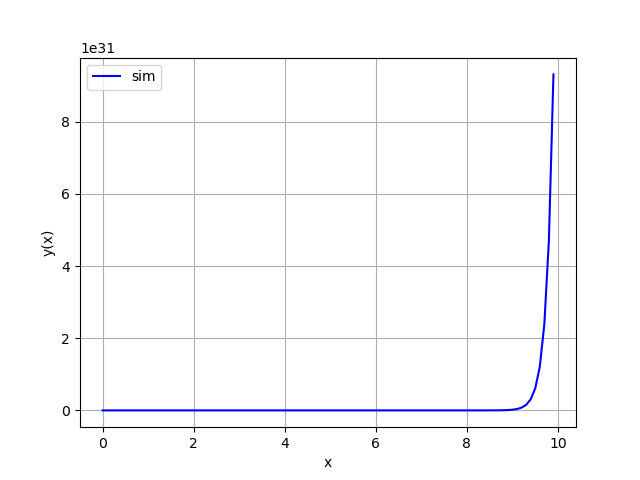
\includegraphics[width=\columnwidth]{figs/fig.png}
\end{figure}
\end{document}
